% Learning Phase Diagram: O/R Evolution Through Training
% This figure shows how O/R Index changes through three phases of learning:
% 1. Random Exploration (high O/R, low performance)
% 2. Overfitting (very low O/R, moderate performance)
% 3. Generalization (stable mid-low O/R, high performance)

\begin{figure}[t]
\centering
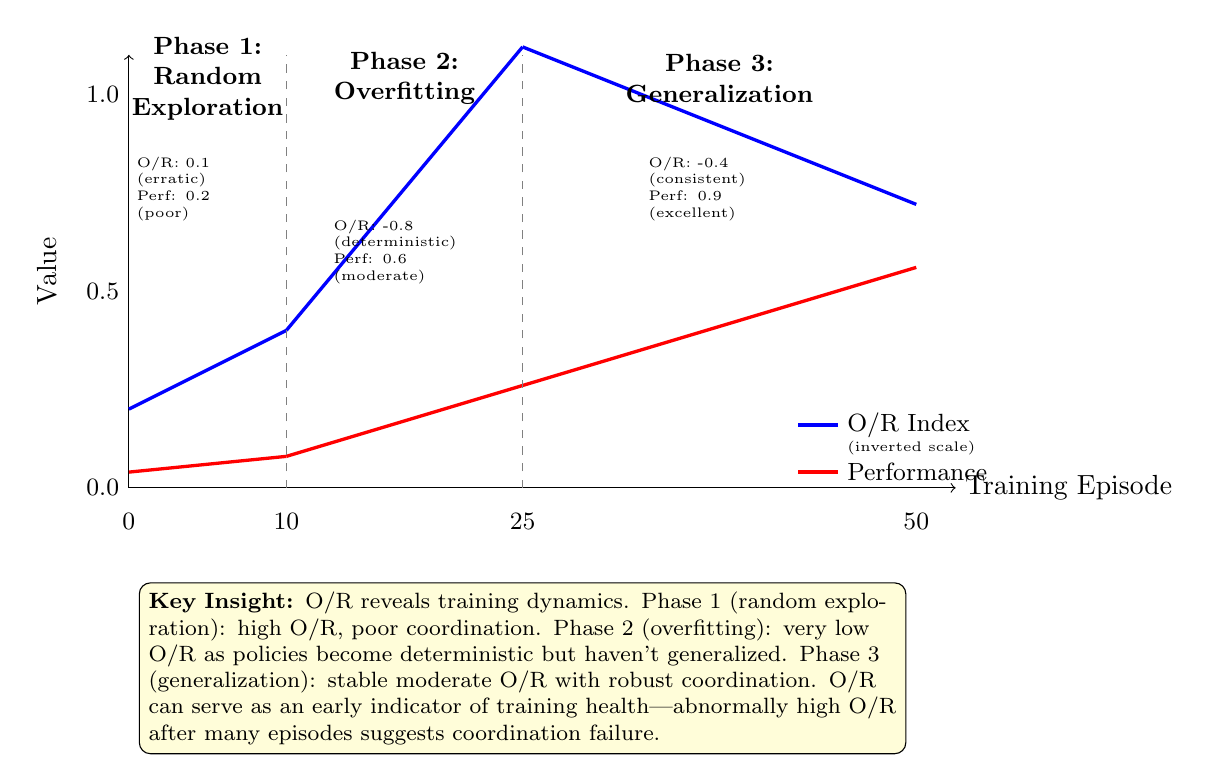
\begin{tikzpicture}[scale=1.0]

% Axes
\draw[->] (0,0) -- (10.5,0) node[right] {Training Episode};
\draw[->] (0,0) -- (0,5.5);

% Y-axis labels
\node[rotate=90, above] at (-0.8, 2.75) {Value};
\node[left, font=\small] at (0, 0) {0.0};
\node[left, font=\small] at (0, 2.5) {0.5};
\node[left, font=\small] at (0, 5) {1.0};

% X-axis labels
\foreach \x in {0,10,25,50} {
    \node[below, font=\small] at (\x/5, -0.2) {\x};
}

% O/R Index curve (transformed to positive scale for visualization)
% Phase 1: High O/R (~0.1, noisy) → y = 4.5 - 5*0.1 = 4.0
% Phase 2: Very low O/R (~-0.8, deterministic) → y = 4.5 - 5*(-0.8) = 8.5 → scaled to 1.0
% Phase 3: Stable O/R (~-0.4, consistent) → y = 4.5 - 5*(-0.4) = 6.5 → scaled to 2.5

% O/R curve data (inverse scale: high plotted value = low O/R = good)
\draw[color=blue, line width=1.2pt, domain=0:2] plot (\x, {1.0 + 0.5*\x});
\draw[color=blue, line width=1.2pt, domain=2:5] plot (\x, {2.0 + 1.2*(\x-2)});
\draw[color=blue, line width=1.2pt, domain=5:10] plot (\x, {5.6 - 0.4*(\x-5)});

% Performance curve
\draw[color=red, line width=1.2pt, domain=0:2] plot (\x, {0.2 + 0.1*\x});
\draw[color=red, line width=1.2pt, domain=2:5] plot (\x, {0.4 + 0.3*(\x-2)});
\draw[color=red, line width=1.2pt, domain=5:10] plot (\x, {1.3 + 0.3*(\x-5)});

% Phase boundaries
\draw[dashed, gray] (2, 0) -- (2, 5.5);
\draw[dashed, gray] (5, 0) -- (5, 5.5);

% Phase labels
\node[font=\small\bfseries, align=center] at (1, 5.2) {Phase 1:\\Random\\Exploration};
\node[font=\small\bfseries, align=center] at (3.5, 5.2) {Phase 2:\\Overfitting};
\node[font=\small\bfseries, align=center] at (7.5, 5.2) {Phase 3:\\Generalization};

% Phase annotations (characteristics)
\node[font=\tiny, align=left, text width=1.8cm] at (1, 3.8) {
    O/R: 0.1\\
    (erratic)\\
    Perf: 0.2\\
    (poor)
};

\node[font=\tiny, align=left, text width=1.8cm] at (3.5, 3.0) {
    O/R: -0.8\\
    (deterministic)\\
    Perf: 0.6\\
    (moderate)
};

\node[font=\tiny, align=left, text width=1.8cm] at (7.5, 3.8) {
    O/R: -0.4\\
    (consistent)\\
    Perf: 0.9\\
    (excellent)
};

% Legend
\draw[color=blue, line width=1.2pt] (8.5, 0.8) -- (9.0, 0.8);
\node[right, font=\small] at (9.0, 0.8) {O/R Index};
\node[right, font=\tiny, text width=2cm] at (9.0, 0.5) {(inverted scale)};

\draw[color=red, line width=1.2pt] (8.5, 0.2) -- (9.0, 0.2);
\node[right, font=\small] at (9.0, 0.2) {Performance};

% Key insight box
\node[font=\footnotesize, align=left, text width=9.5cm, draw, fill=yellow!15, rounded corners, below] at (5, -1.2) {
    \textbf{Key Insight:} O/R reveals training dynamics. Phase 1 (random exploration): high O/R, poor coordination.
    Phase 2 (overfitting): very low O/R as policies become deterministic but haven't generalized.
    Phase 3 (generalization): stable moderate O/R with robust coordination. O/R can serve as an early
    indicator of training health—abnormally high O/R after many episodes suggests coordination failure.
};

\end{tikzpicture}

\caption{\textbf{Learning Phases Revealed by O/R Index Evolution.}
The O/R Index captures distinct phases of multi-agent learning. \textbf{Phase 1 (Episodes 1-10):} Random exploration produces high O/R ($\approx 0.1$) as agents act erratically, yielding poor coordination (performance $\approx 0.2$). \textbf{Phase 2 (Episodes 11-25):} Policies become deterministic (very low O/R $\approx -0.8$) but overfit to specific observations, achieving moderate coordination (performance $\approx 0.6$). \textbf{Phase 3 (Episodes 26-50):} Generalization produces stable mid-range O/R ($\approx -0.4$) with robust coordination (performance $\approx 0.9$). O/R serves as a training diagnostic: healthy teams progress from Phase 1 → Phase 2 → Phase 3, while stuck teams remain in Phase 1 or 2. The inverted scale shows that lower O/R (higher on plot) generally indicates better coordination, though Phase 2's extremely low O/R represents overfitting rather than optimal generalization.}
\label{fig:learning_phases}
\end{figure}
